\section{Un sistema de diagnóstico en CLIPS}

\subsection{Cuestiones 3}

\textbf{1. Analiza el orden de ejecución de las reglas del bloque QUERY RULES y represéntalo gráficamente en forma de árbol.}

\begin{figure}[H]
\centering
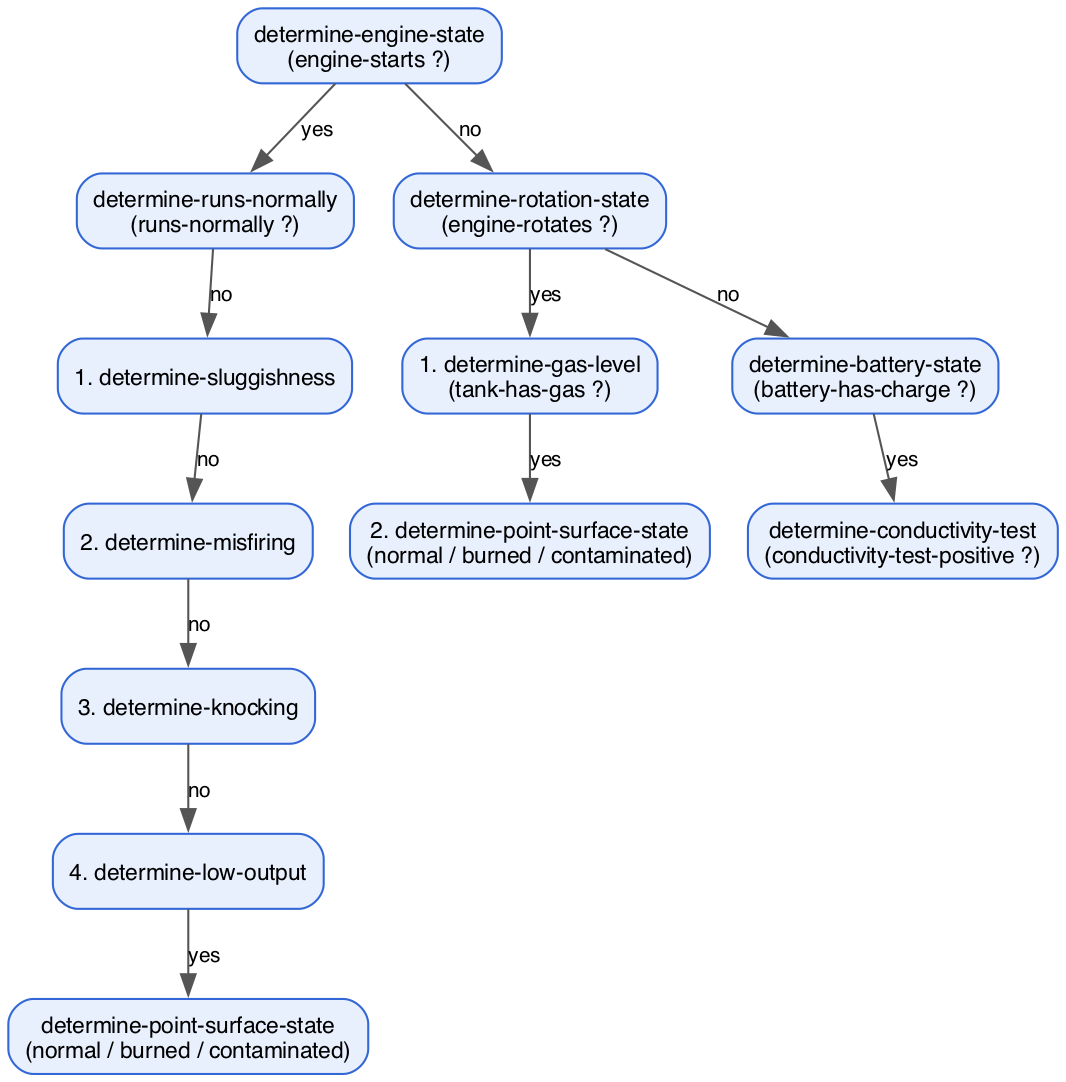
\includegraphics[width=0.8\linewidth]{3_arbol_query_rules.png}
\end{figure}

Cada regla de pregunta afirma un hecho con la respuesta, y ese hecho activa la siguiente pregunta. Cuando un hecho activa varias reglas a la vez, se ejecutan en el orden numerado del árbol. Por ejemplo, \texttt{(runs-normally no)} activa cuatro reglas. Cada rama termina en cuanto se obtiene una reparación.

\textbf{2. Justifica por qué todas las reglas del bloque QUERY RULES incluyen el antecedente (not (repair ?)) y si este es necesario o podría prescindirse de él.}

Hace que solo se pregunte mientras no haya diagnóstico. Varias preguntas pueden estar activadas a la vez. Cuando una respuesta lleva a una reparación, el hecho \texttt{repair} elimina de la Agenda las preguntas pendientes. Por ejemplo, tras ``Add gas'' ya no se pregunta por \texttt{point-surface-state}.

Es necesario, porque sin él el sistema seguiría haciendo preguntas inútiles y podría dar varias reparaciones. En la regla inicial, \texttt{determine-engine-state}, daría igual, ya que al arrancar todavía no se ha podido generar ningún diagnóstico.

\textbf{3. Identifica qué reglas del sistema utilizan la variable saliencia y justifica el papel que juega y los valores elegidos.}

La saliencia es un criterio para seleccionar qué regla del conjunto conflicto se aplica primero, ya que entre las reglas activadas se ejecuta antes la de mayor saliencia. Las reglas que no la declaran tienen saliencia 0, como se ve en la Agenda.

\begin{center}
\small
\begin{tabularx}{\linewidth}{@{}lcY@{}}
\toprule
Regla & Saliencia & Papel \\
\midrule
\texttt{system-banner} & 10 & Muestra el título antes de la primera pregunta. \\
\texttt{print-repair} & 10 & Muestra la reparación en cuanto se obtiene. \\
\texttt{no-repairs} & $-10$ & Diagnóstico por defecto. Solo se ejecuta cuando ya no queda ninguna otra regla, es decir, si no se ha encontrado reparación. \\
\bottomrule
\end{tabularx}
\end{center}

El resto de reglas tiene saliencia 0. Así quedan tres niveles: presentación y resultados (10), razonamiento (0) y conclusión por defecto ($-10$).
